\documentclass[10pt,a4paper]{article}
\usepackage[utf8]{inputenc}
\usepackage[italian]{babel}
\usepackage{amsmath}
\usepackage{amsfonts}
\usepackage{amssymb}
\usepackage{graphicx}
\usepackage[left=2cm,right=2cm,top=2cm,bottom=2cm]{geometry}
\newcommand{\rem}[1]{[\emph{#1}]}

\author{Gruppo AC \\ Federico Belliardo, Francesco Mazzoncini, Giulia Franchi}
\title{Esercitazione N.3: Misure DC su transistor e NOT TTL.}
\begin{document}

\maketitle
\section{Scopo e strumentazione}
Verificare il funzionamento del transistor come amplificatore in un circuito in DC, determinando il guadagno in corrente continua ed analizzare l'uso del transistor in un circuito logico NOT.
\rem{Aggiungere strumentazione}

\section{Identificazione dei terminali dei componenti}

\paragraph{Misura della polarità delle giunzioni del diodo}
Per prima cosa abbiamo analizzando le polarità delle giunzioni del transistor,verificando che si trattasse effettivamente  di un diodo npn ( abbiamo ottenuto valori positivi per le giunzioni BC e BE).

\rem{Tecnicamente questa cosa non è esplicitamente richiesta}
\paragraph{Misura delle resistenze del trimmer}
Utilizzando il multimetro digitale abbiamo misurato le resistenze del trimmer: ai suoi estremi la resistenza è risultata costante $R_{tot}=$, mentre la resistenza tra il terminale intermedio e uno dei due estremi è risultata variabile,più precisamente aumentava  al ruotare in senso orario della vite.
\section{Controllo dello stabilizzatore di tensione}
Abbiamo montato il circuito in  figura \ref{circuito} verificando che  la $V_{out}$ rimanesse costante $5V$ (misurata con multimetro digitale) variando $V{in}$ da 6 a circa  $16V$ e misurando in precedenza le resistenze e il condensatore: $R_L=$  $R_B=$  $C=$
\begin{figure}[!htb]
  \centering
  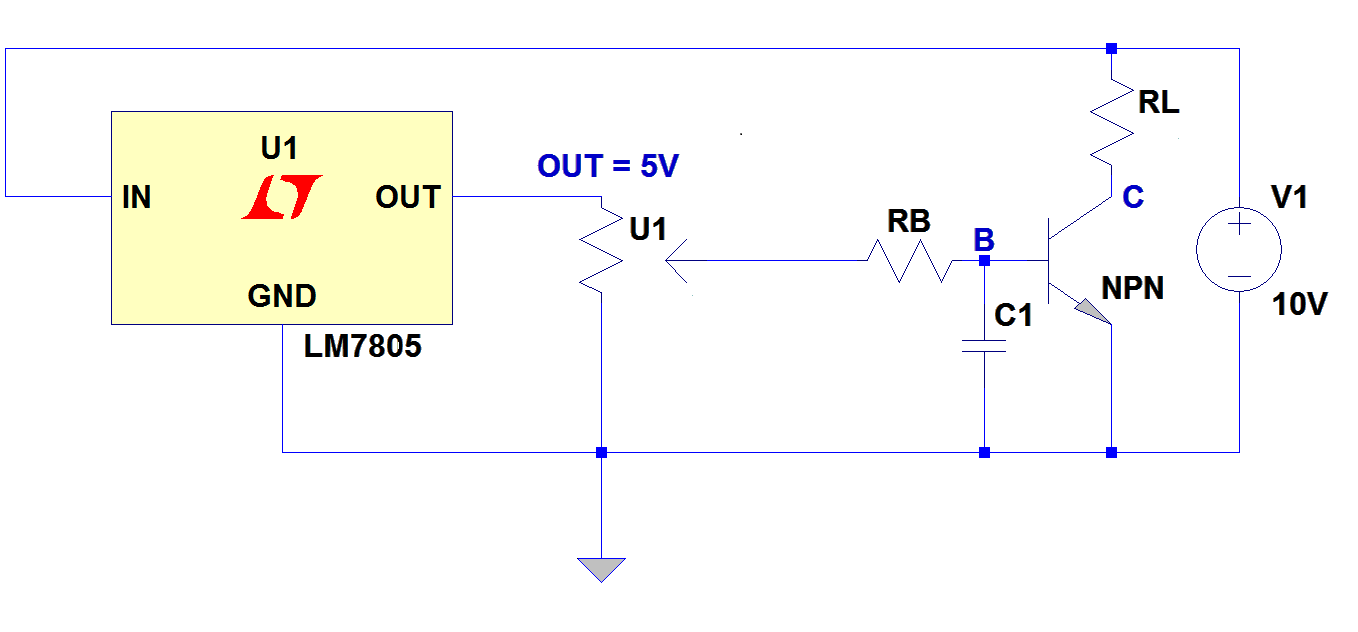
\includegraphics[scale=0.4]{circuito}
\caption{Circuito di amplificazione di correnti continue}
\label{circuito}
\end{figure}
\section{Misure in DC sul transistor}
\paragraph{Calcolo della retta di carico}
Abbiamo collegato il multimetro digitale in parallelo alla resistenza $R_B$  ed i duei canali dell'oscilloscopio ai terminali B e C del transistor. In questo modo siamo stati in grado di misurare contemporaneamente la caduta di tensione $V_{R_B}$ ai capi della resristenza $R_B$, $V_{BE}$ e $V_{CE}$.
\paragraph{Misure sul circuito}
Abbiamo preso varie misure di $V_{R_B}$, $V_{BE}$ e $V_{CE}$  variando la resistenza del potenziometro (ruotando quindi la vite di regolazione). Grazie alle relazioni $I_B=V_{R_B}/R_B$ e $I_C=\frac{V_2-V_{CE}}{R_L}$ abbiamo potuto calcolare la corrente $I_B$ in ingresso alla base e la corrente del collettore $I_C$.
Abbiamo riportato il tutto nella tabella \ref{tabella}
\rem{aggiungi tabella}
\paragraph{Misura del guadagno}
Abbiamo calcolato il guadagno del transistor  eseguendo un fit lineare di $I_C$ e $I_B$ con la  relazione $I_C=h_{FE}I_B+q$.
La massima corrente di collettore erogabile dal transistor è determinata dall'equazione di Kirchoff relativa alla maglia destra del circuito  $V_1 = R_L*I_C + V_{CE}$, quindi il massimo valore di $I_C$ si ha per il minimo valore di $V_{CE}$ che è  approsimativamente $V_{CE}$ in condizioni di saturazione.
  Indichiamo con $V_ {CE_{(SAT)}}$  il massimo valore di $V_{CE}$ per il quale $I_C = I_{C_{(SAT)}}$. Nel caso in esame, osservando la tabella, possiamo  stimare $V_{CE_{(SAT)}}=$. Svolgendo i conti, si trova $I_{C_{MAX}} = $. 
 
 \rem{Secondo me è più sensato misurare Ic e da questa dedurre la corrente di saturazione. La Ic si misura bene dai grafici la I di saturazione è piccola e non sono così convinto che si riesca a stimare bene dalla tabella}
\paragraph{Variazione della retta di carico al variare della tensione di alimentazione.}
 
Abbiamo ruotato la vite regolatrice del trimmer resistivo ottenendo $V_{CE}\simeq 5V$. Fissato quel valore  (facendo sì che $I_B$ restasse costante)  abbiamo misurato $V_{R_L}$ ai capi di $R_L$ con il multimetro digitale  e $V_{CE}$ tramite l'oscilloscopio al variare di $V_1$ tra $6 V$ e $16 V$. Tali dati sono riportati in tabella insieme a quelli di $I_C=V_{R_L}/R_L$.

%Questo ci permette di costruire una curva caratteristica del diodo a corrente di base costante. Questa può essere fittata da una legge esponenziale del tipo:
%$I_c = I_s e^{\frac{V_{BE}}{V_T}} (1-e^{-\frac{V_{CE}}{V_T}}$ quando il transisto è polarizzato in saturazione o in diretta è circa costante duqnue la curva da un andamento esponenziale che uò essere fittato. IL coeffiente che compare davanti alla curva esponenziale è esattamente il coefficiente hfe * I_b che è legato al valore asistotico dellla corrente I_c.
 
\section{Uso del transistor in un circuito logico NOT }
\paragraph{Montaggio del circuito}
Abbiamo montato il circuito rappresentato in  figura \ref{circuito2}.
\begin{figure}[!htb]
  \centering
 %TODO Aggiungere tutte le label su immagini e tabelle
  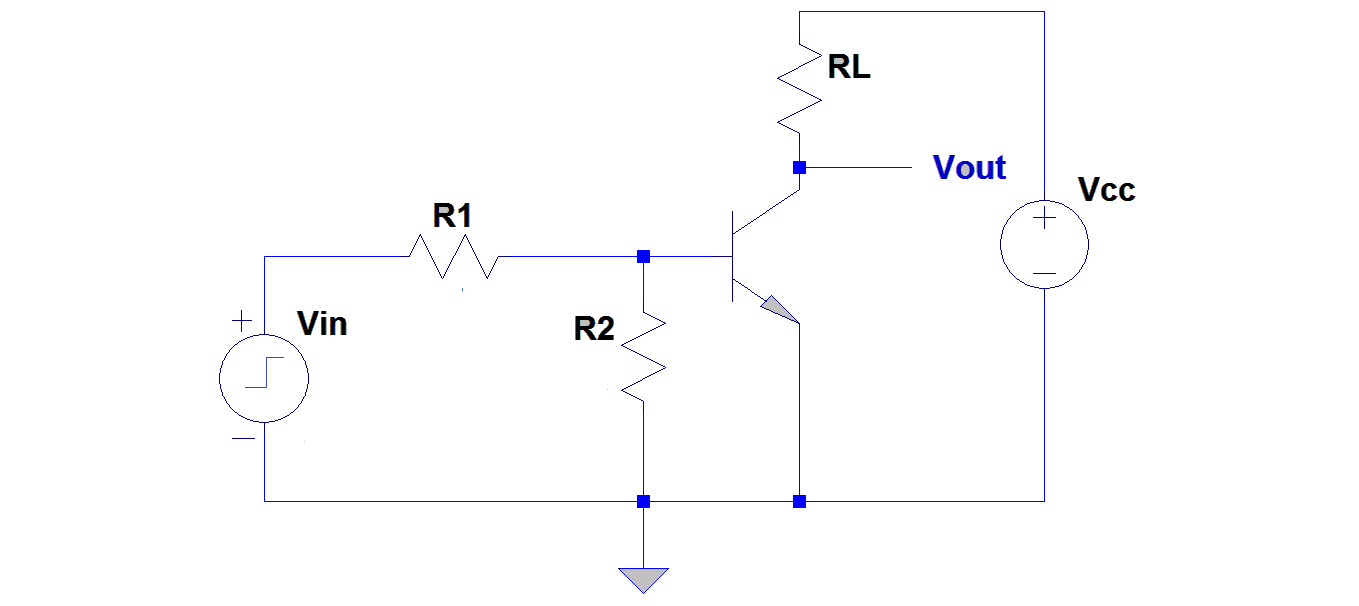
\includegraphics[scale=0.4]{circuito2} \label{circuito2}
\caption{Circuito logico NOT}
\label{circuito2}
\end{figure} 

In ingresso abbiamo collegato  il generatore di funzioni in modalità output pulse, il quale genera un’onda quadra oscillante tra $0 V$ e $5 V$. Abbiamo usato  il generatore di tensione $V_{CC}=$, con un valore scelto in modo tale da far funzionare il transistor  in regime di saturazione e di interdizione al variare di $V_{in}$. Le resistenze usate ( misurate con un multimetro digitale ) sono : $R_1=$ $R_2=$ $R_L=$

\paragraph{Verifica del corretto funzionamento del circuito}
\paragraph{Misura dei tempi di transizione di $V_{out}$ }

\paragraph{Discussione sui tempi di transizione di$ V_{out}$}

\end{document} 